\section{Optymalizacja dla dużych ekranów}

Ze względu na różnorodność urządzeń mobilnych oczekuje się zwykle od dostępnych aplikacji, aby były do nich przystosowane. Wykorzystanie identycznego wyglądu na wszystkich zwykle się nie sprawdza, ponieważ komponenty mogą być zbyt ściśnięte, rozciągnięte lub też ucięte, co nie wygląda estetycznie. Z tego powodu postanowiono dokonać optymalizacji wyglądu tworzonego rozwiązania dla urządzeń o większych rozmiarach, czyli tabletów. 

Optymalizacji dokonano dwoma prostymi metodami. Pierwsza polegała na zastosowaniu dwukolumnowego układu dla znajdujących się w aplikacji list. Przykład jednej z nich przedstawiono na rysunku \ref{fig:tablet} w części (a). Pozwala to znacznie lepiej wykorzystać dostępne na ekranie miejsce. Druga metoda polega na dodaniu bocznych marginesów, co jest widoczne na tym samym rysunku w części (b). Powoduje to powstanie pustej przestrzeni, którą można by lepiej zagospodarować, lecz poprawia walory estetyczne. 

\begin{figure}[ht]
  \captionsetup[subfigure]{justification=centering}
  \centering
  \begin{subfigure}[t]{0.32\textwidth}
    \centering
    \fbox{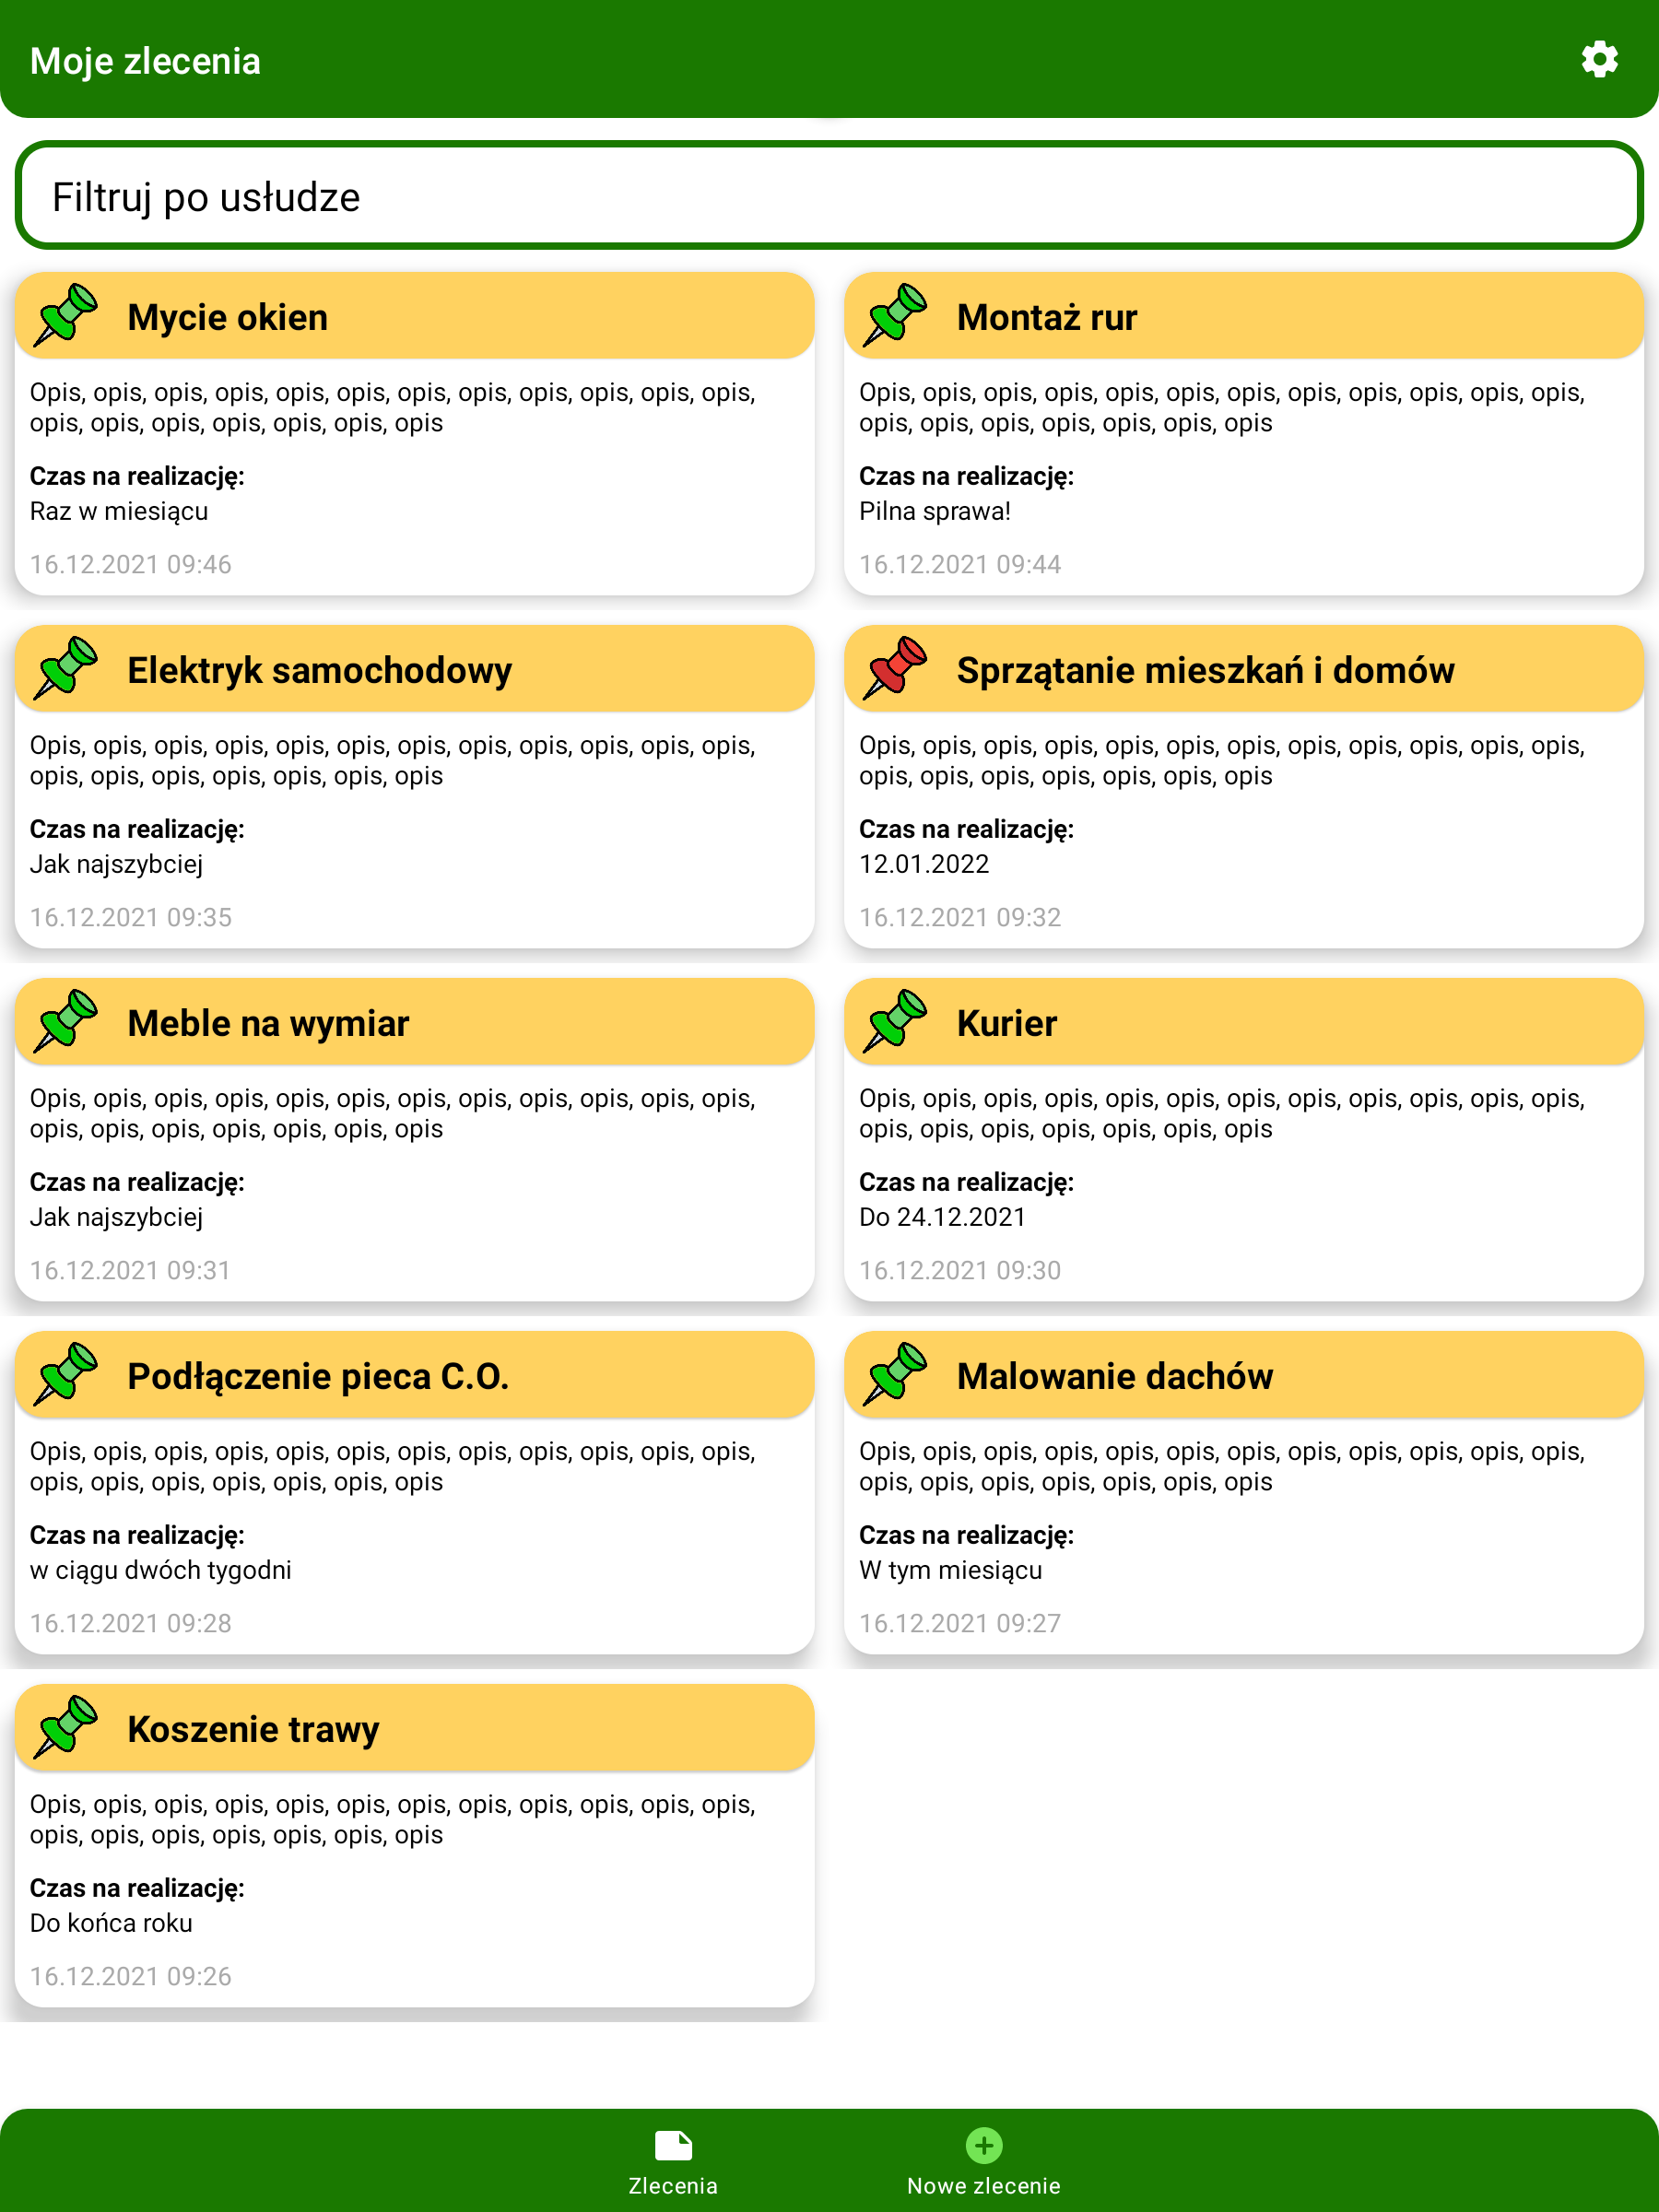
\includegraphics[width=0.97\linewidth]{screens/tablet_jobs.png}}
    \caption{Ekran listy zleceń klienta}
  \end{subfigure}
  \begin{subfigure}[t]{0.50\textwidth}
    \centering
    \fbox{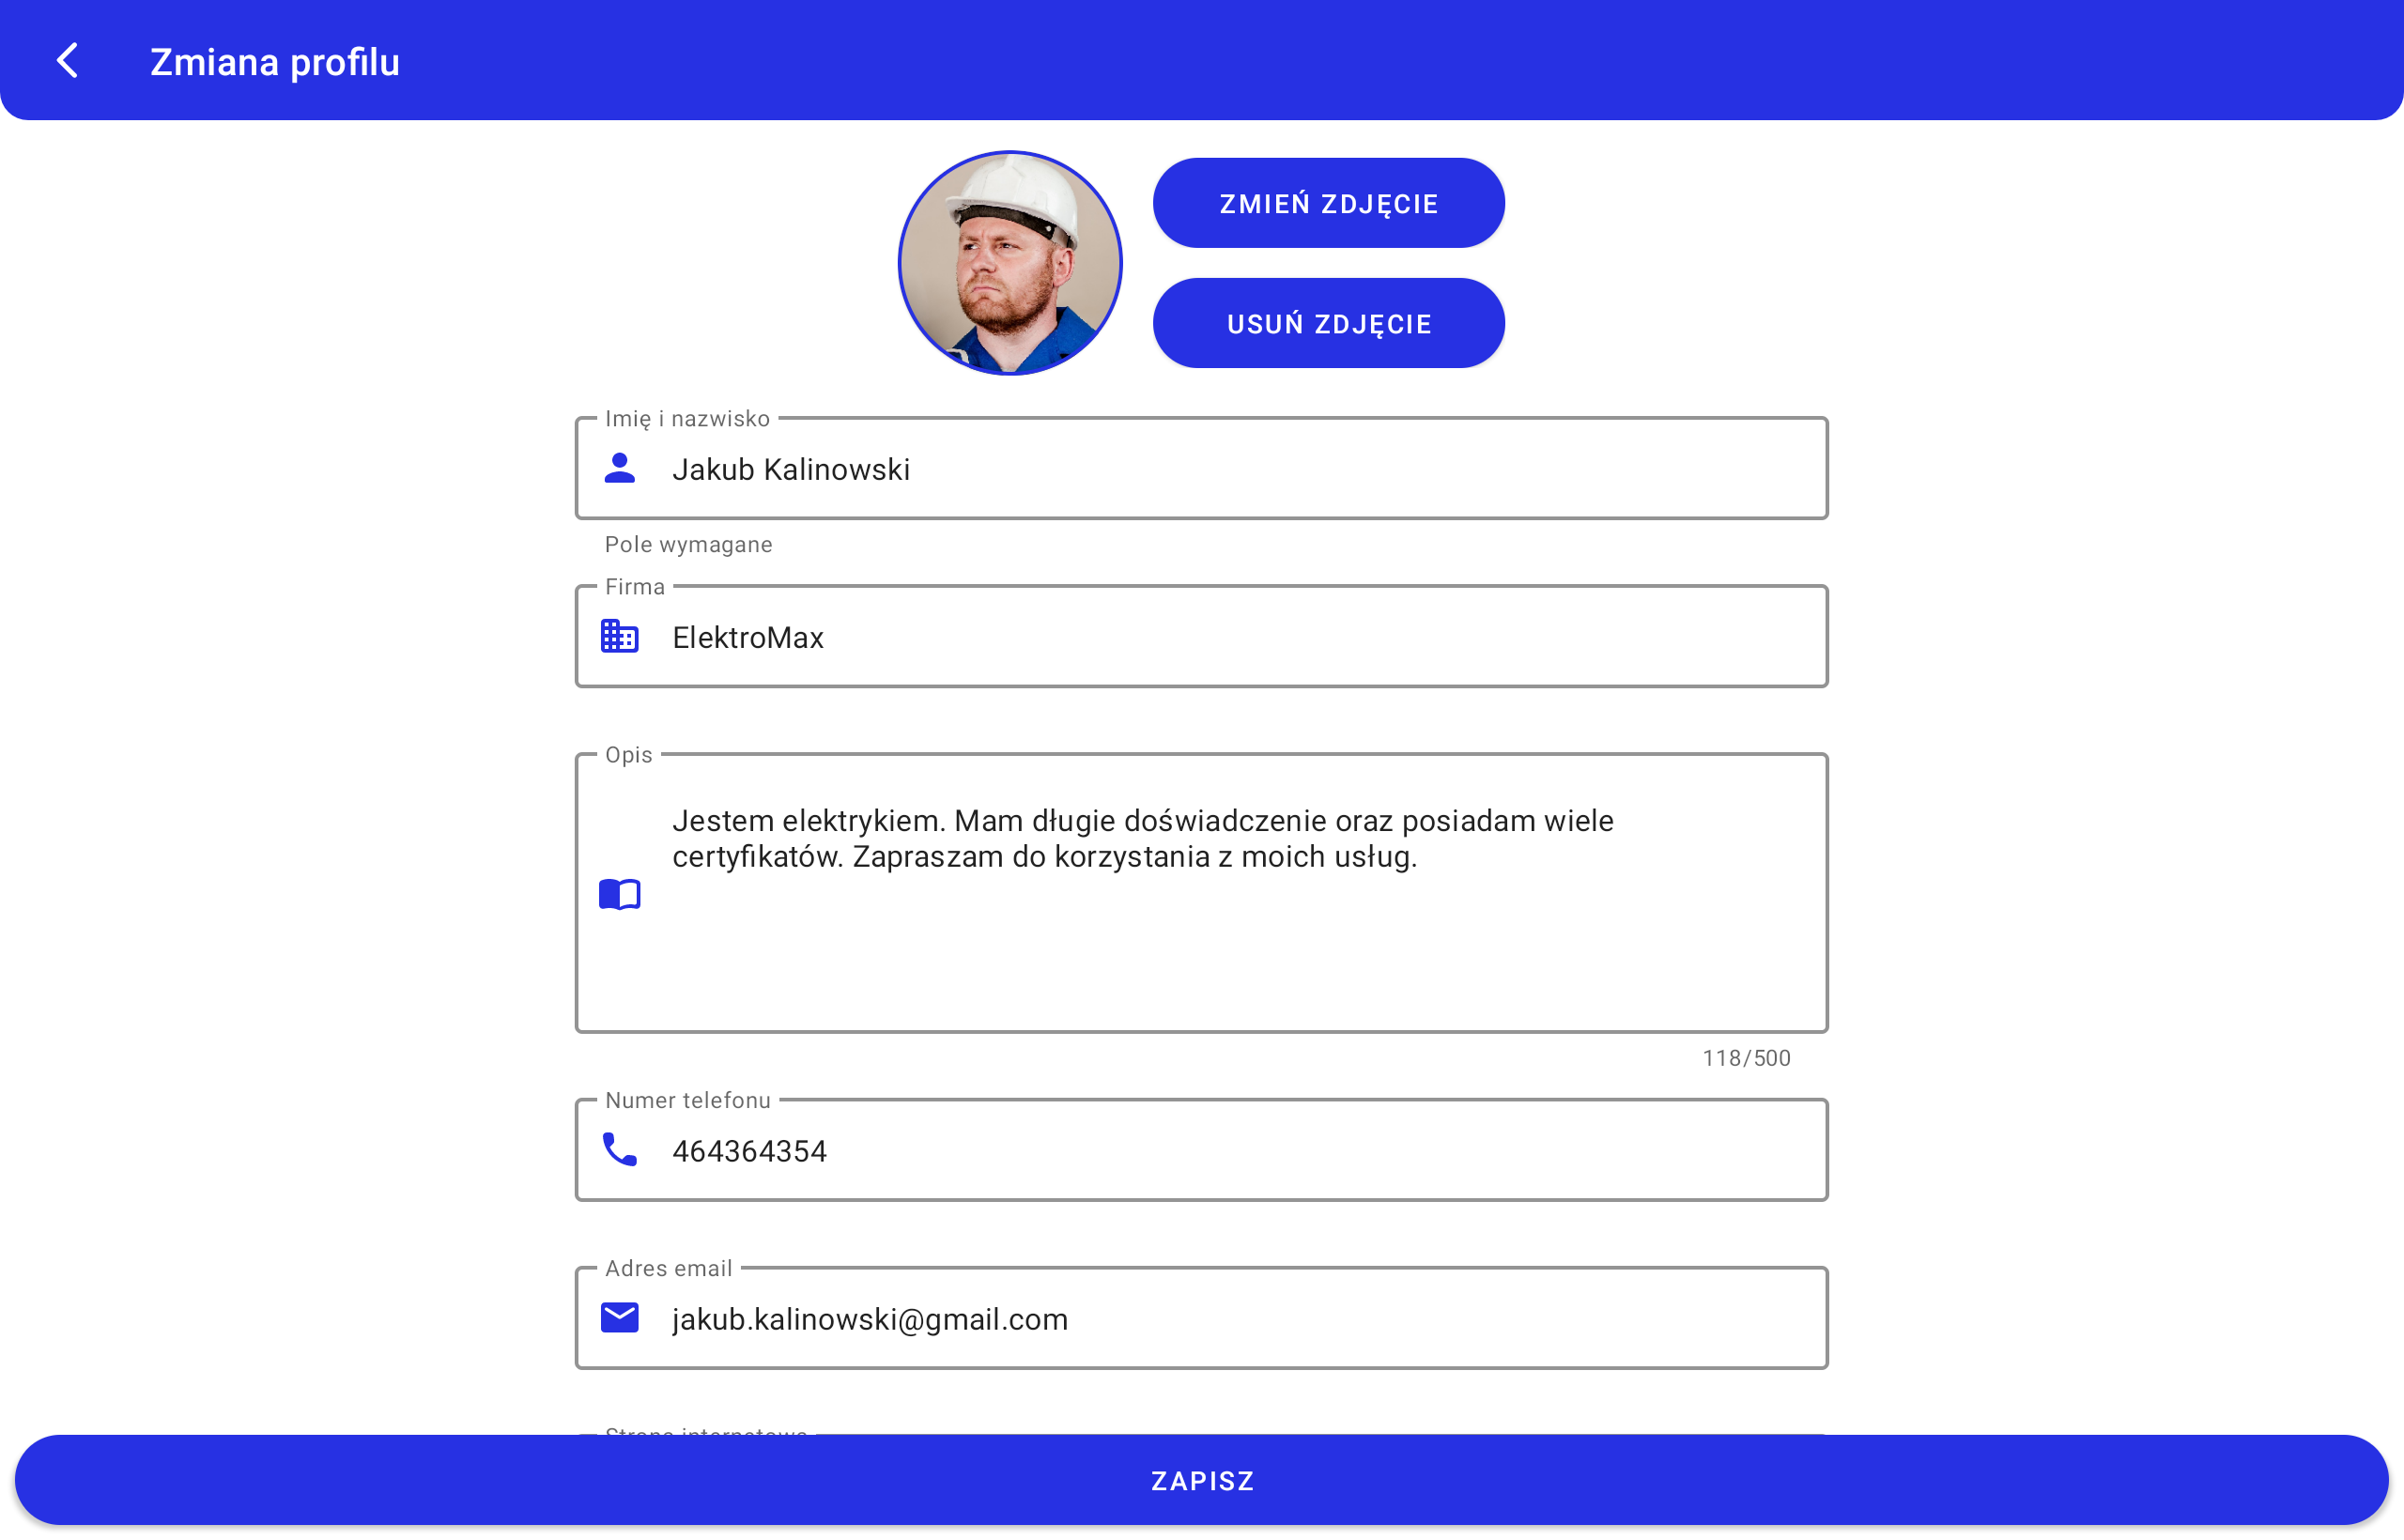
\includegraphics[width=0.97\linewidth]{screens/tablet_info.png}}
    \caption{Ekran edycji profilu wykonawcy}
  \end{subfigure}
  \caption{Widok aplikacji na tablecie}
  \label{fig:tablet}
\end{figure}

% Dostosowania wyglądu można dokonać bardziej szczegółowo, nie uznano tego jednak za konieczne. O znacznie mniejszej liczbie użytkowników tabletów, w porównaniu z telefonami, świadczyć może strona Statcounter \cite{statcounter}. Analizuje ona ruch sieciowy i można się z niej dowiedzieć, że w Polsce mają one ponad pięćdziesiąt razy mniejszy udział w rynku niż telefony. Z tego powodu postanowiono skupić się na bardziej potrzebnych i mniej czasochłonnych funkcjonalnościach.

Z uwagi na brak posiadania przez autora odpowiednio dużego urządzenia fizycznego, by zaobserwować zmianę interfejsu, szczególnie przydatne okazały się emulatory dostarczane wraz ze środowiskiem Android Studio. Dzięki nim możliwe było dokładne przetestowanie nowego wyglądu na kilku tabletach o różnych rozmiarach.